

\actTitle{Worksheet 3.2}

\noindent \textbf{Instructions:}  Work together in groups of  3 or 4 to complete the following problems.

Student goals:
\begin{itemize}
  \item Use the definition of an exponential function to define a
    function describing a situation given in written, verbal, or
    graphical form.
  \item Use the properties and operations of exponential functions to
    solve for any variable in an expression that has exponential functions.
  \item Be able to graph exponential functions. Be able to compare and
    identify different exponential functions whose parameters differ.
  \item Given the parameters associated with multiple exponential
    grow/decay equations determine the general behaviour and compare
    the relative growth or decay of the different equations.
  \item Determine the equation for the balance of a bank account or
    credit debt for compound interest given a written description of
    the situation.
  \item Determine the equation for the value of an exponential
    growth/decay problem given a written description of the
    situation. Be able to identify if a situation results in either
    growth or decay.
\end{itemize}



\subsection{Exponential Functions}
\begin{enumerate}
\item Which of the following equations represent exponential
  functions?
  {Circle the exponential functions.}
  $$f(x)=2x+1, \quad
  g(x)=-4^x, \quad
  h(x)=1^x, \quad
  j(x)=3\cdot 2^x,  \quad
  m(x)=x^2,  \quad
  p(x)=\left(\frac{3}{10}\right)^{x+3}.$$

\item Write two examples of exponential growth functions.
\vfill

\item Write two examples of exponential decay functions.
\vfill

\item Fill in the table of values for the function $j(x)=3\cdot 2^x$.

\begin{center}
%\renewcommand{\arraystretch}{2}
\begin{tabular}{|r|l|}
\hline
\textbf{$x$} & \textbf{$j(x)$~~} \\ \hline
-2           &                 \\ [0.5em] \hline
-1           &                 \\ [0.5em] \hline
0            &                 \\ [0.5em] \hline
1            &                 \\ [0.5em] \hline
2            &                 \\ [0.5em] \hline
\end{tabular}
\end{center}

\clearpage

\item A parent function and a sequence of operations is given in each
  part below. For each part make a sketch of the parent function,
  determine the new function, and sketch the new function. \textbf{Briefly
  describe the long-term behaviour of each function.}

  \begin{enumerate}
  \item $g(x)=3^x$
    \sideNote{State the new function obtained in each step
        of the transformation below.}

        \begin{tabular}{m{0.5\textwidth}m{0.5\textwidth}}

            \begin{enumerate}
            \item Shift 4 units to the left.
              \vspace{3em}
            \item Reflect across the $y$-axis.
              \vspace{3em}
            \item Shift upward 2 units.
              \vspace{3em}
            \end{enumerate}


          & 


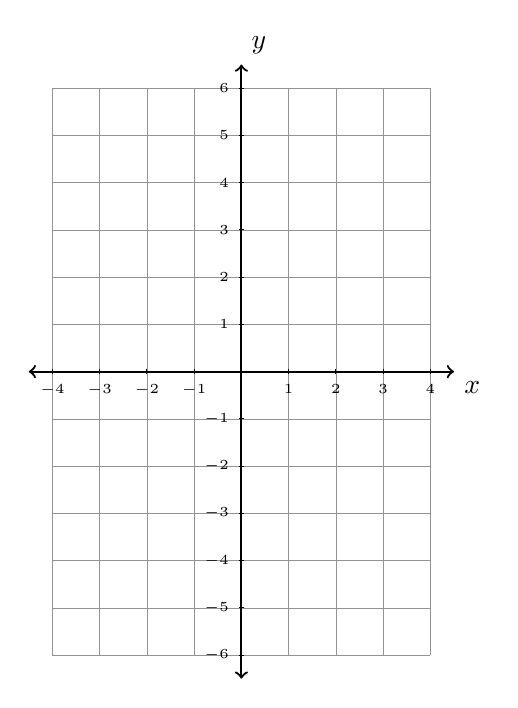
\begin{tikzpicture}[y=.6cm, x=.6cm,font=\sffamily,
	mydot/.style={
    circle,
    fill=white,
    draw,
    outer sep=0pt,
    inner sep=1.5pt
  }]
    %% Add a grid
    \draw[step = 1, gray, very thin,opacity=0.85] (-4, -6) grid (4, 6);
 	%% Draw the axes
	\draw[thick,<->] (-4.5,0) -- coordinate (x axis mid) (4.5,0) node[anchor = north west] {$x$};
    \draw[thick,<->] (0,-6.5) -- coordinate (y axis mid) (0,6.5) node[anchor = south west] {$y$};
    %% Label the y axis
    \foreach \y in {-6,...,-1,1,2,...,6} {
      \draw (1pt, \y) -- (-1pt, \y) node[anchor =  east] {\tiny$\y$};
    }
    %% Label the x axis
    \foreach \x in {-4,...,-1,1,2,...,4} {
      \draw (\x,1pt) -- (\x,-1pt) node[anchor = north] {\tiny$\x$};
    }

  \end{tikzpicture}


\end{tabular}

\vfill


\item $\displaystyle g(x)=\left(\frac{1}{3}\right)^x$

  \begin{tabular}{m{0.5\textwidth}m{0.5\textwidth}}

      \begin{enumerate}
      \item Shift 1 unit to the left.
        \vspace{3em}
      \item Stretch horizontally by a factor of 4.
        \vspace{3em}
      \item Reflect across the $x$-axis.
        \vspace{3em}
      \end{enumerate}


    &
              

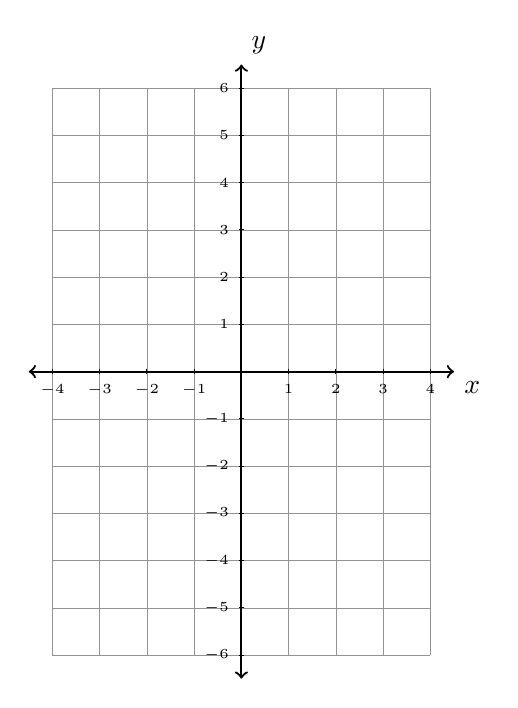
\begin{tikzpicture}[y=.6cm, x=.6cm,font=\sffamily,
	mydot/.style={
    circle,
    fill=white,
    draw,
    outer sep=0pt,
    inner sep=1.5pt
  }]
    %% Add a grid
    \draw[step = 1, gray, very thin,opacity=0.85] (-4, -6) grid (4, 6);
 	%% Draw the axes
	\draw[thick,<->] (-4.5,0) -- coordinate (x axis mid) (4.5,0) node[anchor = north west] {$x$};
    \draw[thick,<->] (0,-6.5) -- coordinate (y axis mid) (0,6.5) node[anchor = south west] {$y$};
    %% Label the y axis
    \foreach \y in {-6,...,-1,1,2,...,6} {
      \draw (1pt, \y) -- (-1pt, \y) node[anchor =  east] {\tiny$\y$};
    }
    %% Label the x axis
    \foreach \x in {-4,...,-1,1,2,...,4} {
      \draw (\x,1pt) -- (\x,-1pt) node[anchor = north] {\tiny$\x$};
    }

  \end{tikzpicture}

      
  \end{tabular}


\vfill


\end{enumerate}

\clearpage
\subsection{Solving Exponential Equations}
Solving an equation means to find the set of values that can be
substituted for the variable, creating a true statement.


\textbf{Example.} To solve the equation, $\sqrt[3]{x}=3$ we need to
undo the operations happening to $x$.  Remember,
$\sqrt[3]{x}=x^{1/3}$.

\begin{equation*}
  \begin{array}{rcl@{\hspace{2em}}l}
    \sqrt[3]{x} & = & 3 & \textrm{Original~equation.}\\
    x^{1/3} & = & 3 & \textrm{Use~definition~of~cube~root.}\\
    \left(x^{1/3}\right)^{3/1} & = & 3^{3/1} & \textrm{Raise~both~sides~to~$3/1$.}\\
    x^1 & = & 3^3 & \textrm{Use~exponential~properties.} \\
    x & = & 27    & \textrm{Simplify.}
  \end{array}
\end{equation*}

\item Use the example above to solve each of the following
  equations. Take one step at a time and write down each step.
\begin{enumerate}
\item  $\left(\sqrt{x}\right)^{3}=64$. 
  \vfill
\item  $5\sqrt[7]{x}-2=13$
  \vfill
\end{enumerate}




\clearpage
\subsection{Compound Interest}


\noindent The compound interest formula is
$$A(t)=P\left(1+\frac{r}{n}\right) ^{nt},$$
where $P$ is the initial principal, $r$ is the annual compounded
interest rate (a number between 0 and 1), $n$ is the number of
compounding periods per year, and $t$ is the time in years.

\item If \$10,000 is invested at an annual rate of 8\%, determine the
  amount present after 10 years given the following:

\begin{enumerate}
\item Compounded annually\vfill
\item Compounded monthly \vfill
\item Compounded weekly \vfill
\item Compounded daily \vfill
\item Compounded hourly \vfill
\item Compounded every minute \vfill
\item Compounded continuously\vfill
\end{enumerate}

What is the general trend, and how do the results relate to one
another?

\clearpage

\subsection{Laws of Exponents} ~

\noindent
\fbox{
  \parbox{\dimexpr 0.6\linewidth}%
  {
    \noindent
    Laws of Exponents \\
    \begin{equation*}
      \begin{array}{rcl@{\hspace{4em}}rcl}
        a^m \cdot a^n & = & a^{m+n}  & \left(\dfrac{a}{b}\right)^n & = & \dfrac{a^n}{b^n} \\ [20pt]
        (a^m)^n & = & a^{mn}  &  \dfrac{a^m}{a^n} & = & a^{m-n} \\ [20pt]
        (ab)^n & = & a^nb^n &  \dfrac{1}{a^n} & = & a^{-n}
      \end{array}
    \end{equation*}
  }
}



\item Simplify the expressions completely (there should only be one
  instance of each variable and only positive exponents). For each
  step, identify the rule used to simplify.

\begin{enumerate}
\item $\left(\dfrac{x}{y}\right)^{-9}\cdot y^{10}$

  \vfill

\item $\left(-2x^3y\right)^5 \left(\dfrac{x^9}{5y^2}\right)$

  \vfill

\item $\dfrac{\sqrt{x^4y^3}}{y}$

  \vfill

\item $\sqrt{x^2+4}$

  \vfill

\end{enumerate}


\clearpage

\item Two functions are defined,
  \begin{equation*}
    \begin{array}{rcl@{\hspace{2em}}rcl}
      p(x) & = & \left(\frac{1}{2}\right)^{x}, & d(x) & = & a^x,
    \end{array}
  \end{equation*}
  where $a$ is a positive constant.
  \begin{enumerate}
  \item Make a rough sketch of the function $p(x)$. (Label your axes.)
    \vfill
  \item Determine all possible values of $a$ that will ensure that
    $p(x)>d(x)$ for all $x>0$.
    \vfill
  \item Determine all possible values of $a$ that will ensure that
    $p(x)>d(x)$ for all $x<0$.
    \vfill
  \item Determine all possible values of $a$ that will ensure that
    $p(x)<d(x)$ for all $x>0$.
    \vfill
  \end{enumerate}



\end{enumerate}


\hwTitle{Section 3.2}

\begin{enumerate}
  \item  Match each of the following functions to their graph.
\begin{multicols}{2}
\begin{enumerate}
	\item $y=2^x$
	\item $y=-2^x$
	\item $y=2^{-x}$
	\item $y=-2^{-x}$
	\item $y=1.25^x$
	\item $y=1.25^{-x}$
	\item $y=-1.25^x$
	\item $y=-1.25^{-x}$
\end{enumerate}	
\end{multicols}
%\begin{center}
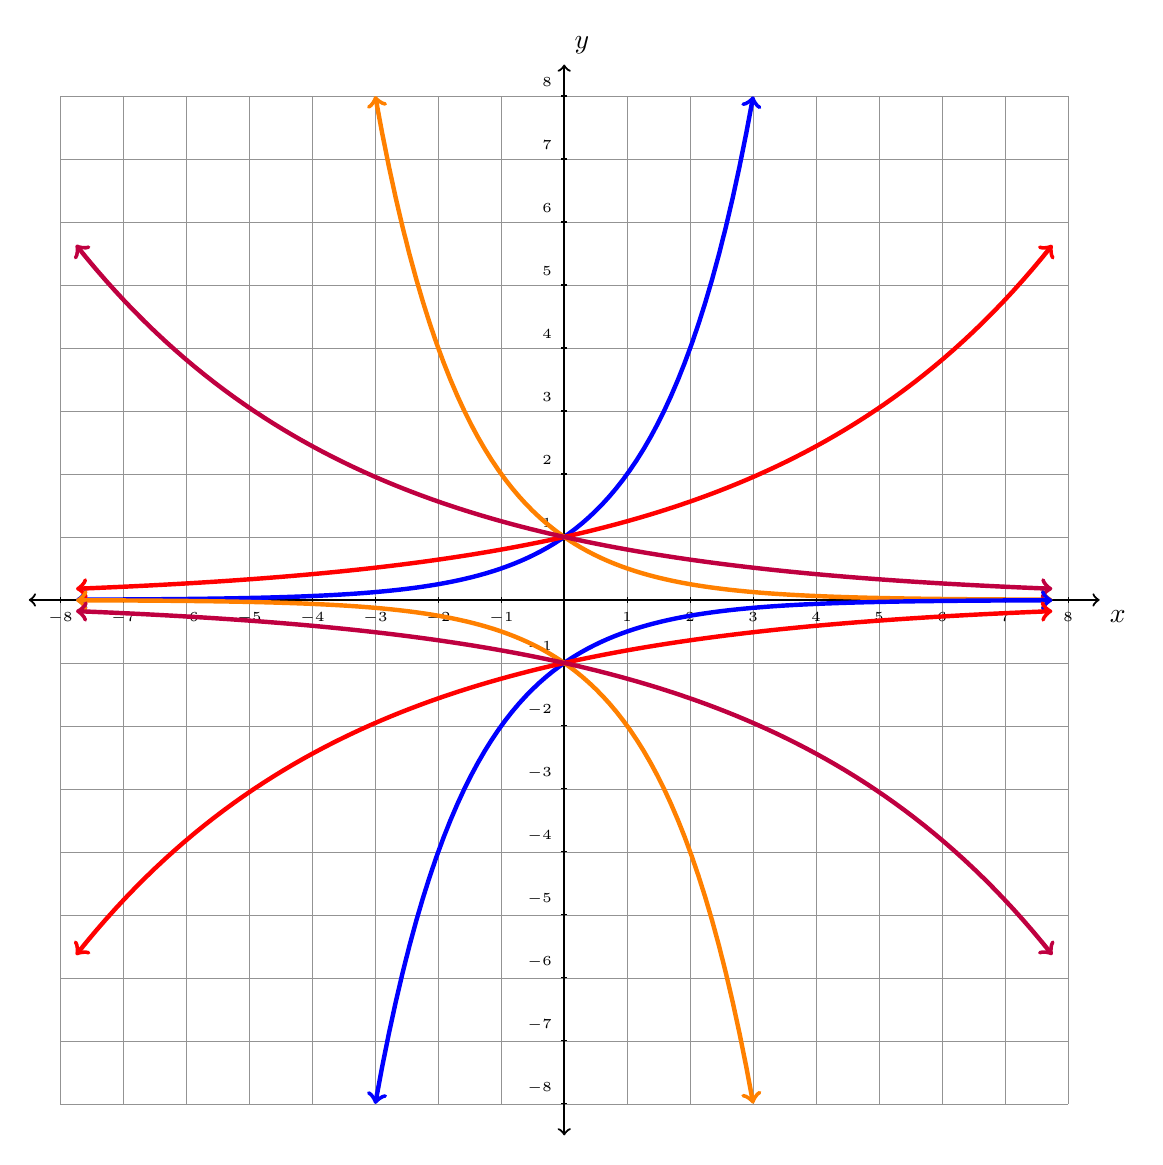
\begin{tikzpicture}[y=.8cm, x=.8cm,font=\sffamily,
	mydot/.style={
    circle,
    fill=white,
    draw,
    outer sep=0pt,
    inner sep=1.5pt
  }]
    %% Add a grid
    \draw[step = 1, gray, very thin,opacity=0.85] (-8, -8) grid (8, 8);
 	%% Draw the axes
	\draw[thick,<->] (-8.5,0) -- coordinate (x axis mid) (8.5,0) node[anchor = north west] {$x$};
    \draw[thick,<->] (0,-8.5) -- coordinate (y axis mid) (0,8.5) node[anchor = south west] {$y$};
    %% Label the y axis
    \foreach \y in {-8,...,-1,1,2,...,8} {
      \draw (1pt, \y) -- (-1pt, \y) node[anchor = south east] {\tiny $\y$};
    }
    %% Label the x axis
    \foreach \x in {-8,...,-1,1,2,...,8} {
      \draw (\x,1pt) -- (\x,-1pt) node[anchor = north] {\tiny $\x$};
    }
    %% Draw the function.
    \begin{scope}
%         \draw[very thick,blue] (-3,2) -- (1,1);
%         \draw[very thick,blue] (3.05,1.05) -- (4,3);
%         \draw[very thick,blue] (1.1,4) -- (3,4);
    %semi-circle
         %\draw[very thick, blue] (1,1) arc [radius=1, start angle=180, end angle= 5];
     %parabola
         %\draw[ultra thick, blue, domain=-5:0] plot (\x, {(-0.2)*(\x-5)*(\x+5)});
         \draw[ultra thick, blue, <->, domain=-7.75:3.0] plot[samples=100] (\x, {2^\x});
         \draw[ultra thick, red, <->, domain=-7.75:7.75] plot[samples=100] (\x, {(1.25)^\x});
         \draw[ultra thick, orange, <->, domain=-3.0:7.75] plot[samples=100] (\x, {2^-\x});
         \draw[ultra thick, purple, <->, domain=-7.75:7.75] plot[samples=100] (\x, {(1.25)^-\x});
         \draw[ultra thick, blue, <->, domain=-3.0:7.75] plot[samples=100] (\x, {-2^-\x});
         \draw[ultra thick, red, <->, domain=-7.75:7.75] plot[samples=100] (\x, {-(1.25)^-\x});
         \draw[ultra thick, orange, <->, domain=-7.75:3.0] plot[samples=100] (\x, {-2^\x});
         \draw[ultra thick, purple, <->, domain=-7.75:7.75] plot[samples=100] (\x, {-(1.25)^\x});
           %dots
%         \fill[blue] (-3, 2) circle[radius=0.5ex];
%         \fill[blue] (1,1) circle[radius=0.5ex];
%         \fill[blue] (4,3) circle[radius=0.5ex];
%         \draw[very thick, blue] (3,1) circle[radius=0.5ex];
%         \fill[blue] (3,4) circle[radius=0.5ex];
%         \draw[very thick, blue] (1,4) circle[radius=0.5ex];


    \end{scope}

    %%\node[above=0.1cm] at (-2,2 )   {\nextXValue};

\end{tikzpicture}
%\end{center}

\item Solve each of the following equations for $x$.
  \begin{enumerate}
  \item $\left(\sqrt{x}\right)^3=8$
  \item $\left(\sqrt[3]{x}\right)^2=16$
  \item $\left(\sqrt[9]{x}\right)^5=243$
  \item $\left(\sqrt[4]{x}+2\right)^3=27$
  \item $\left(\frac{\sqrt[3]{x}-2}{7}\right)^4=16$
  \end{enumerate}
\item Simplify the expressions completely (there should only be one
  instance of each variable and only positive exponents). For each
  step, identify the rule used to simplify.
  \begin{enumerate}
  \item $\dfrac{x^{8/3}y^{3/5}}{x^2}$
  \item $\left( \dfrac{-2x^{-3}}{y^{12} }  \right)^{2/5}$
  \item $x^3 \cdot (2x)^2$
  \item $\dfrac{(\sqrt{x}(x-1))^{100} \cdot x^2}{(x-1)^{101}}$ 
  \item $\sqrt{x^2}$
  \end{enumerate}

\item The function $Gi(x)$ is defined by
  \begin{eqnarray*}
    Gi(x) & = & 5-C \cdot \left(\frac{1}{6}\right)^x,
  \end{eqnarray*}
  where $C$ is a constant.
  \begin{enumerate}
  \item Given that $Gi(0)=3.5$, determine the value of $C$.
  \item Make a rough sketch of the function, $Gi(x)$. Describe the
    behaviour of $Gi$, and in particular discuss the long-term trend
    of the function.
  \end{enumerate}

\item The function $Ro(x)$ is defined by
  \begin{eqnarray*}
    Ro(x) & = & A + 7 \cdot \left(\frac{2}{3}\right)^x,
  \end{eqnarray*}
  where $A$ is a constant.
  \begin{enumerate}
  \item Given that $Ro(0)=2.1$, determine the value of $A$.
  \item Make a rough sketch of the function, $Ro(x)$. Describe the
    behaviour of $Gi$, and in particular discuss the long-term trend
    of the function.
  \end{enumerate}

\item Two functions are defined,
  \begin{equation*}
    \begin{array}{rcl@{\hspace{2em}}rcl}
      u(x) & = & \left(\frac{5}{7}\right)^x, & w(x) & = & a^x,
    \end{array}
  \end{equation*}
  where $a$ is a constant.
  \begin{enumerate}
  \item Make a rough sketch of the function $u(x)$. (Label your axes.)
  \item Determine all possible values of $a$ that will ensure that
    $u(x)>w(x)$ for all $x>0$.
  \item Determine all possible values of $a$ that will ensure that
    $u(x)>w(x)$ for all $x<0$.
  \end{enumerate}

\item Two functions are defined,
  \begin{equation*}
    \begin{array}{rcl@{\hspace{2em}}rcl}
      c(x) & = & \left(\frac{1}{3}\right)^x, & k(x) & = & a^x,
    \end{array}
  \end{equation*}
  where $a$ is a constant.
  \begin{enumerate}
  \item Make a rough sketch of the function $c(x)$. (Label your axes.)
  \item Determine all possible values of $a$ that will ensure that
    $c(x)<k(x)$ for all $x>0$.
  \item Determine all possible values of $a$ that will ensure that
    $c(x)<k(x)$ for all $x<0$.
  \end{enumerate}
  


\end{enumerate}
